\documentclass{article}
\usepackage{graphicx}
\usepackage{ragged2e}
\usepackage{geometry}
\title{Experimentation}
\author{Vigneswaran Chandrasekaran}
\date{10-11-2019}

\begin{document}
\section{Ablation studies}
The proposed work's superior performance is contingent upon various novel components and to visualize the contribution of each one, ablation analysis was carried out.
\subsection{Performance with/without using Information Theory}

\subsection{Performance with/without using Novel parameter updation}
To understand the criticality of Novel parameter updation step mentioned in section[] while pre-training, the ablation study was conducted. Firstly, instead of using the proposed parameter updation step (Eq 19 and 20), Eq[] were used, in which the loss factor was assigned with simple euclidean distance between best bin [] and $k^{th}$ bin. 
\\
$ W_{k,j}^{new} = W_{k,j}^{old} - \eta1/2\sqrt{(M^{i}_{k} - M^{i}_{best})^2}$, where $\eta$ is the decay parameter identical to [] in Eqn [] \& []. Without any other changes the model was evaluated using MNIST dataset. 
Figure [] shows the rate of change of loss with\&without using the proposed parameter updation. 
\\
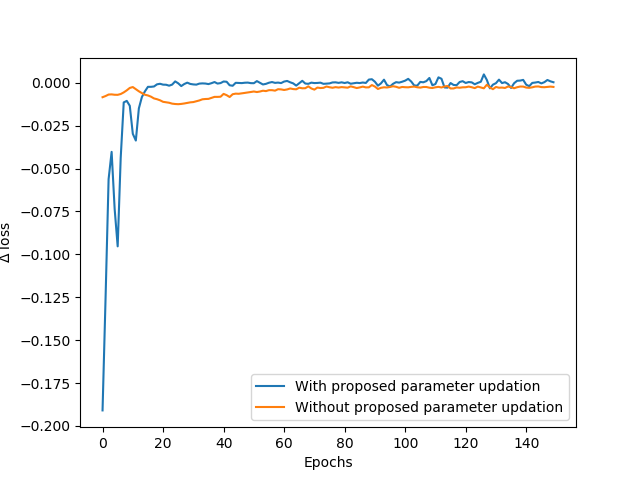
\includegraphics[width=10cm, height = 6cm]{param_upd_ab.png}
\subsection{Performance with/without using K-Helly property}


\end{document}

